\documentclass{ximera}

\title{Courses}
\author{Bart Snapp}

\begin{document}
\onecolumn
\begin{multicols}{2}
\begin{abstract}
    Combine Ximera activities to make courses.
\end{abstract}
\maketitle
% \onecolumn
% \begin{multicols}{2}
This section is about ``best practices'' when writing a book
\begin{itemize}
    \item Keep related content in the same folder
    \item use \texttt{\textbackslash sectionstyle} and
          \texttt{\textbackslash chapterstyle}
    \item When you give a definition, ask a question after.
    \item When you give and example, give an explanation, with
          \texttt{\textbackslash answer} boxes to fill in.
    \item Think about how you name things
    \item Think about how paths are resolved.
\end{itemize}


\begin{example}
    \begin{verbatim} 
%% where to look for inputs
\makeatletter
\def\input@path{
{./}
{./coverArt/}
{./introduction/}
}
\makeatother   
\end{verbatim}
\end{example}

\end{multicols}


\begin{center}
    \scalebox{.7}{
    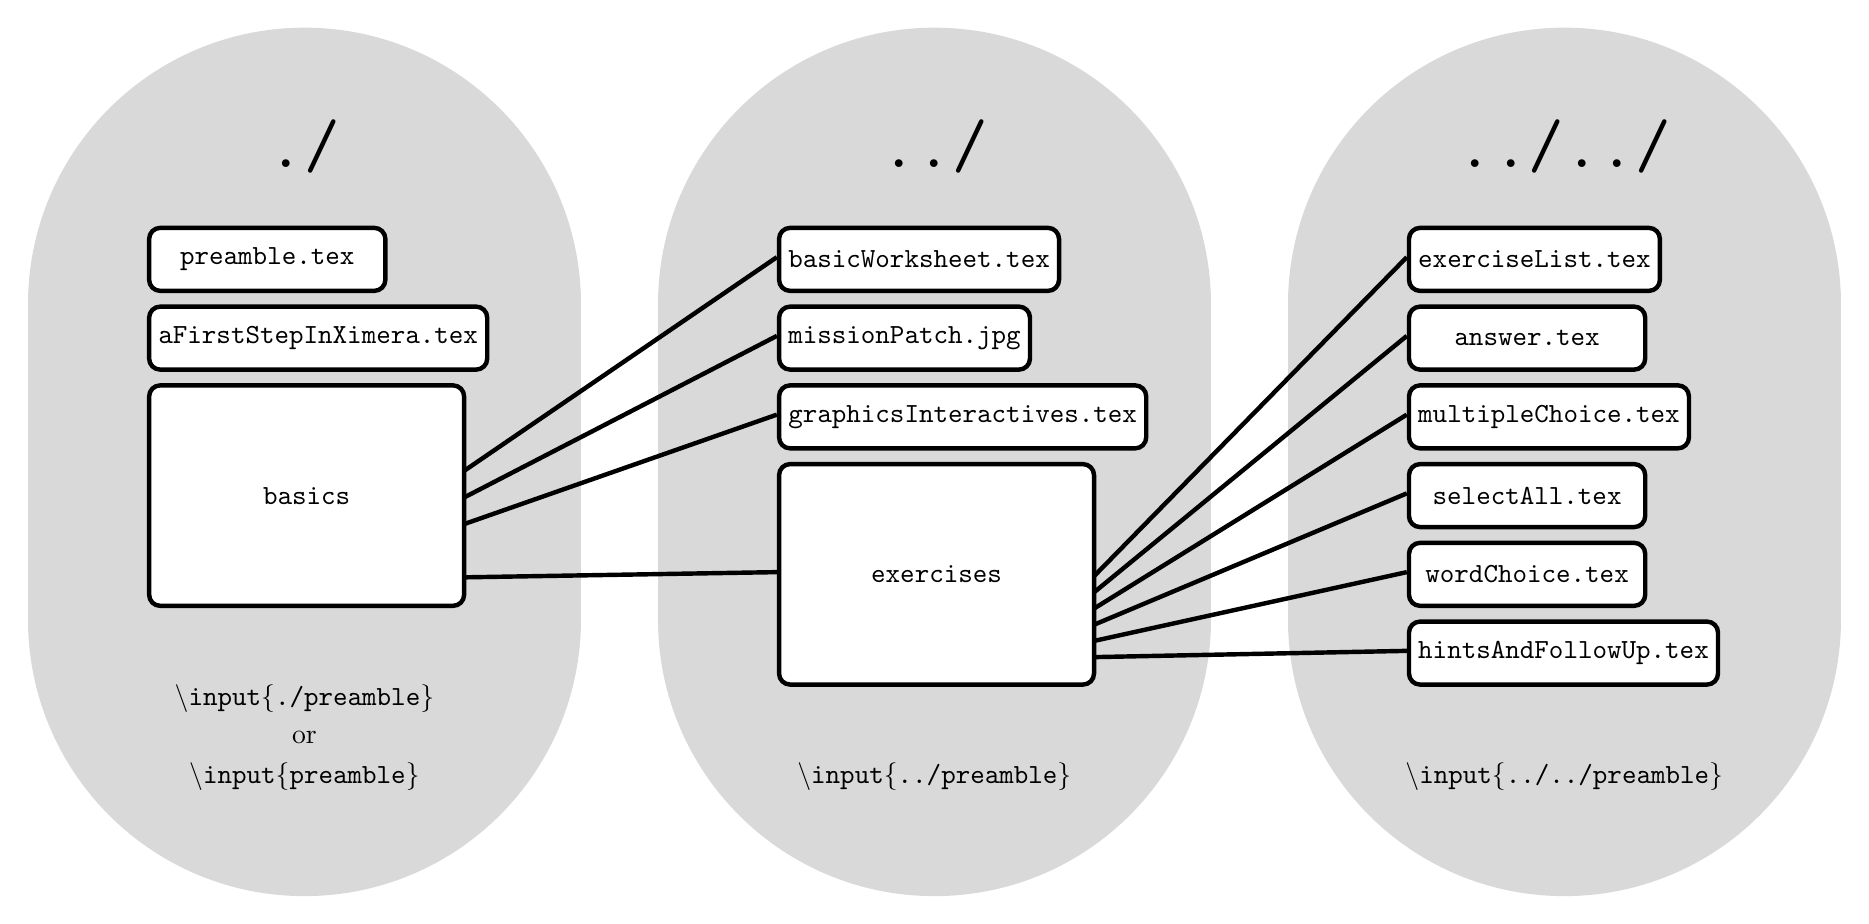
\begin{tikzpicture}
      % Define styles for nodes
      \tikzstyle{document} = [anchor=north west,draw, rounded corners, rectangle,
      minimum width=3cm,fill=white, minimum height=.8cm, ultra
      thick,font=\ttfamily]
      \tikzstyle{folder} = [anchor=north west,draw, rectangle, rounded corners,
      minimum width=4cm,fill=white, minimum height=2.8cm, ultra
      thick,font=\ttfamily]
  
      % Thick grey lines
      \draw[line width=200pt,white!85!black,line cap=round] (2,2) -- (2,-2);
      \draw[line width=200pt,white!85!black,line cap=round] (10,2) -- (10,-2);
      \draw[line width=200pt,white!85!black,line cap=round] (18,2) -- (18,-2);
  
      % Connections
      \draw[ultra thick] (2,-1.5) -- (8,2.6);
      \draw[ultra thick] (2,-1.5) -- (8,1.6);
      \draw[ultra thick] (2,-1.5) -- (8,.6);
      \draw[ultra thick] (2,-1.5) -- (8,-1.4);
  
      \draw[ultra thick] (11,-2.5) -- (16,2.6);
      \draw[ultra thick] (11,-2.5) -- (16,1.6);
      \draw[ultra thick] (11,-2.5) -- (16,.6);
      \draw[ultra thick] (11,-2.5) -- (16,-.4);
      \draw[ultra thick] (11,-2.5) -- (16,-1.4);
      \draw[ultra thick] (11,-2.5) -- (16,-2.4);
  
      % Symbols at top
      \node at (2,4) {\Huge \tt ./};
      \node at (10,4) {\Huge \tt ../};
      \node at (18,4) {\Huge \tt ../../};
  
      % Define the folders at top level
      \node[document] at (0,3) {preamble.tex};
      \node[document] at (0,2) {aFirstStepInXimera.tex};
      \node[folder] at (0,1) {basics};
  
      % Define the documents in the basics folder
      \node[document] at (8,3) {basicWorksheet.tex};
      \node[document] at (8,2) {missionPatch.jpg};
      \node[document] at (8,1) {graphicsInteractives.tex};
      \node[folder] at (8,0) {exercises};
  
      % Define the documents in the exercises folder
      \node[document] at (16,3) {exerciseList.tex};
      \node[document] at (16,2) {answer.tex};
      \node[document] at (16,1) {multipleChoice.tex};
      \node[document] at (16,0) {selectAll.tex};
      \node[document] at (16,-1) {wordChoice.tex};
      \node[document] at (16,-2) {hintsAndFollowUp.tex};
  
      % paths at bottom
      \node at (2,-3) {\tt\textbackslash input\{./preamble\}};
      \node at (2,-3.5) {or};
      \node at (2,-4) {\tt\textbackslash input\{preamble\}};
      \node at (10,-4) {\tt\textbackslash input\{../preamble\}};
      \node at (18,-4) {\tt\textbackslash input\{../../preamble\}};
  \end{tikzpicture}}
  \end{center}
\twocolumn


NOTE -- I think the input path is AUTOMATICALLY part of the graphics path.
Please CHECK
\begin{example}
    \begin{verbatim}
%% where to find images
\graphicspath{  
{./}
{./graphicsVideosAndInteractives/}
}    
\end{verbatim}
\end{example}









\end{document}